\documentclass[11pt,a4paper]{article}

\usepackage[margin=2.5cm]{geometry}
\usepackage{amsmath,amssymb,bm}
\usepackage{graphicx}
\usepackage{booktabs}
\usepackage{hyperref}
\usepackage{float}
\usepackage{caption}

\title{Exploration of 3D Scene Reconstruction from RGB-D Data:\\
From Pinhole Geometry to TSDF Fusion in a Webots Simulation}

\author{Haoyang Zhou \and Kaiyu Li}
\date{\today}

\begin{document}
\maketitle

\begin{abstract}
This paper studies the complete pipeline of reconstructing a 3D scene from
RGB-D data. Starting from the pinhole camera model derived with similar
triangles, we show how a depth measurement turns an RGB image into an RGB-D
image, and how every pixel can be back-projected into a colored 3D point cloud.
We then analyze why a single frame only covers the visible side of a scene,
introduce camera poses to align multiple frames into one world frame, and
address the fusion of multiple noisy point clouds with a truncated signed
distance field (TSDF), from which a triangle mesh is extracted by marching
cubes. All steps are validated on a dataset captured with a simulated RGB-D
camera in Webots: the pinhole intrinsics predicted by geometry match the
simulator values within $0.1\%$, the reconstructed floor matches the true
plane within $3\,\mathrm{mm}$ RMS, and the fused mesh reproduces the true
scene extent exactly. Ablation studies show that TSDF fusion outperforms naive point-cloud
concatenation as depth noise and pose noise grow, and quantify the trade-off
between voxel size, reconstruction quality and runtime.
\end{abstract}

\begin{figure}[H]
\centering
\begin{minipage}{0.48\linewidth}
\centering
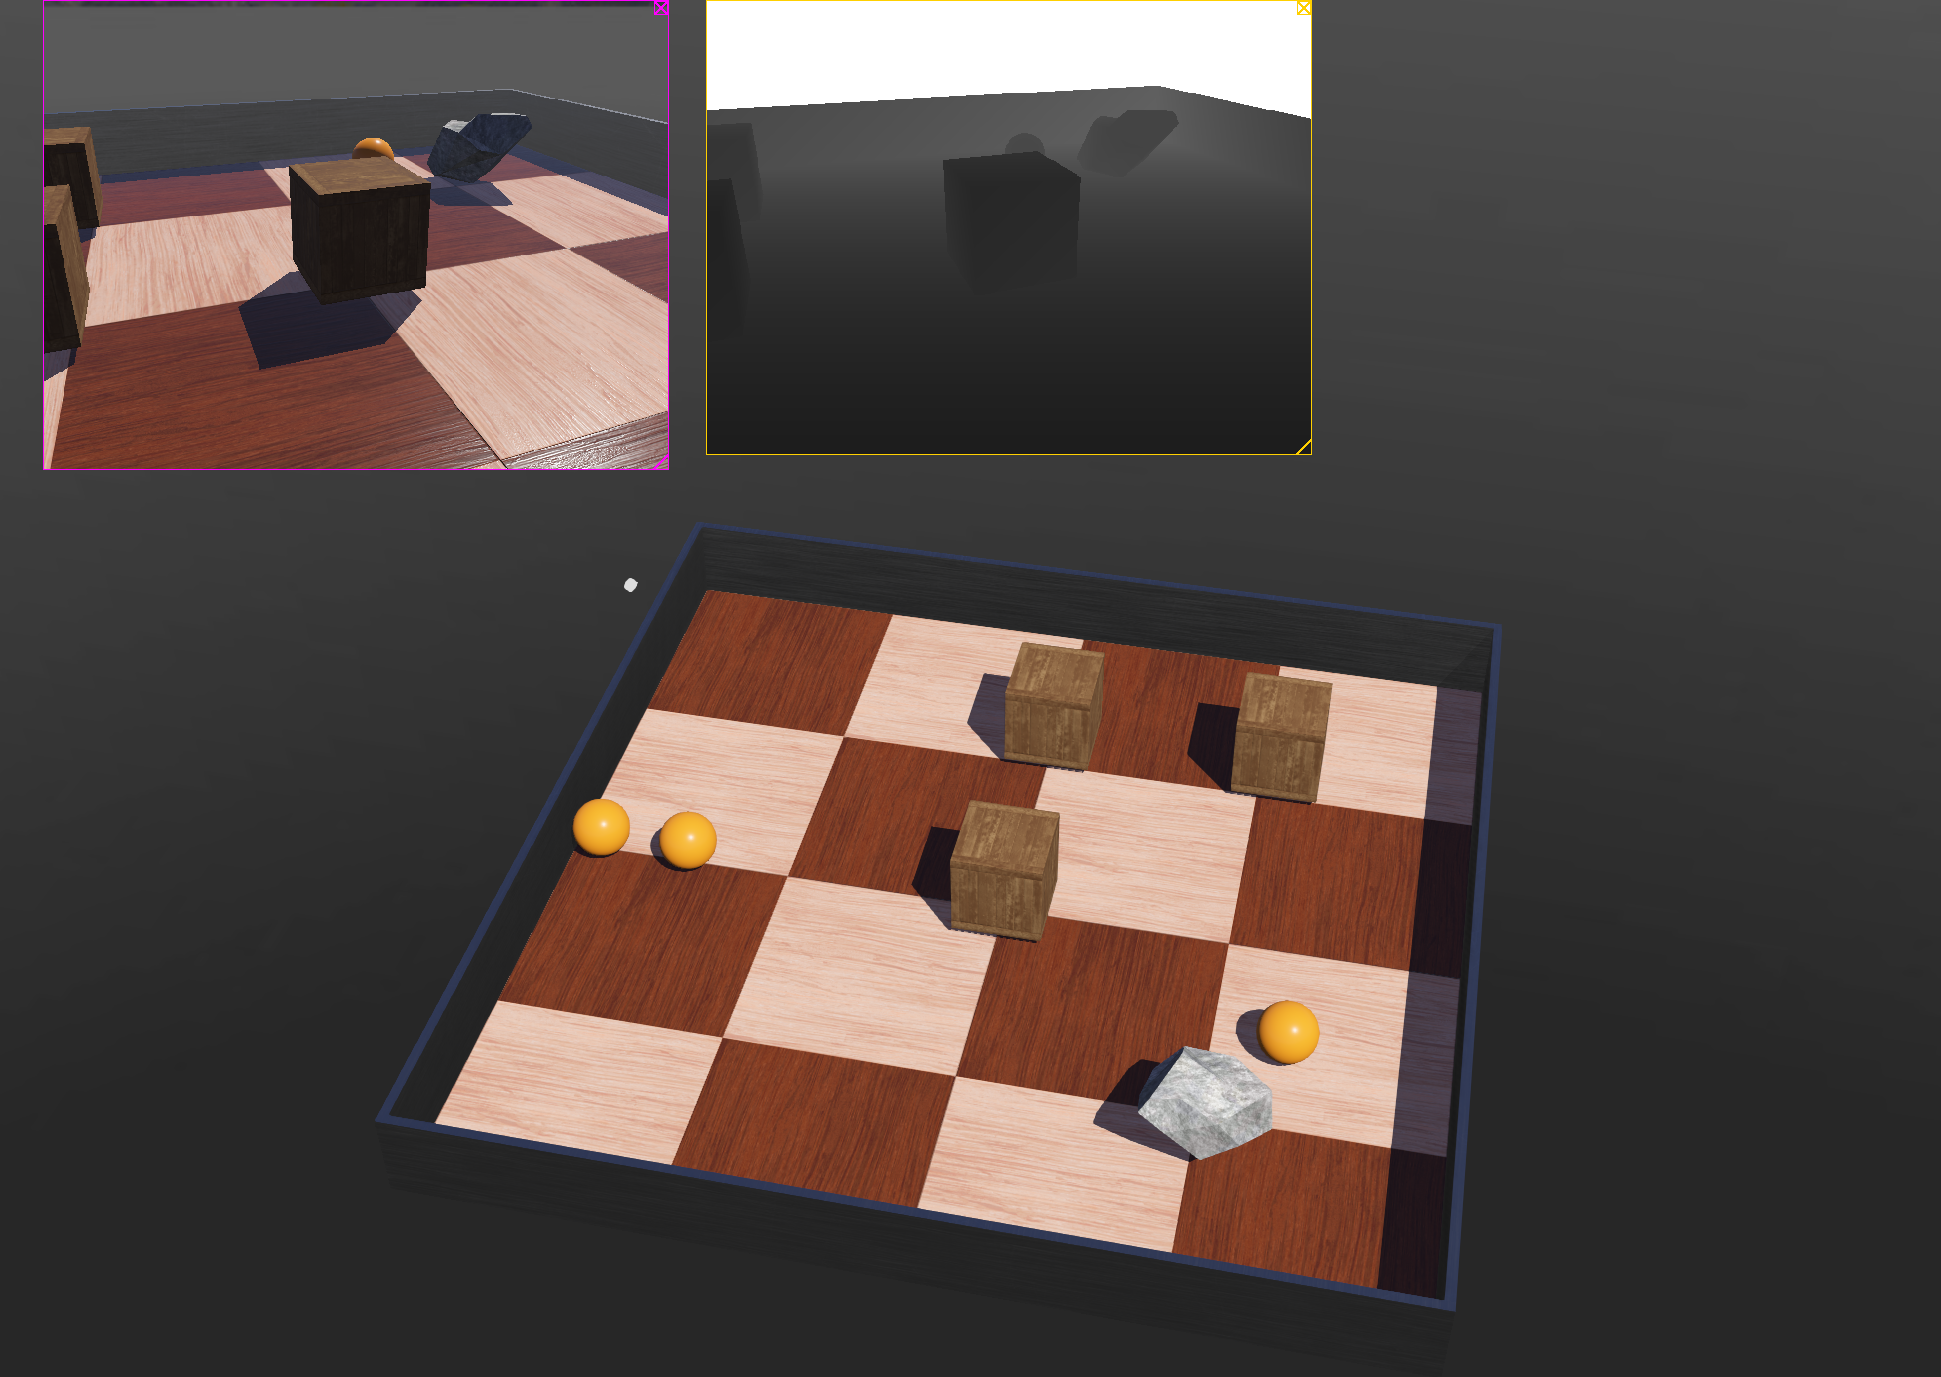
\includegraphics[width=\linewidth]{figures/fig_world.png}\\
(a) pixel-aligned RGB-D capture in Webots
\end{minipage}\hfill
\begin{minipage}{0.48\linewidth}
\centering
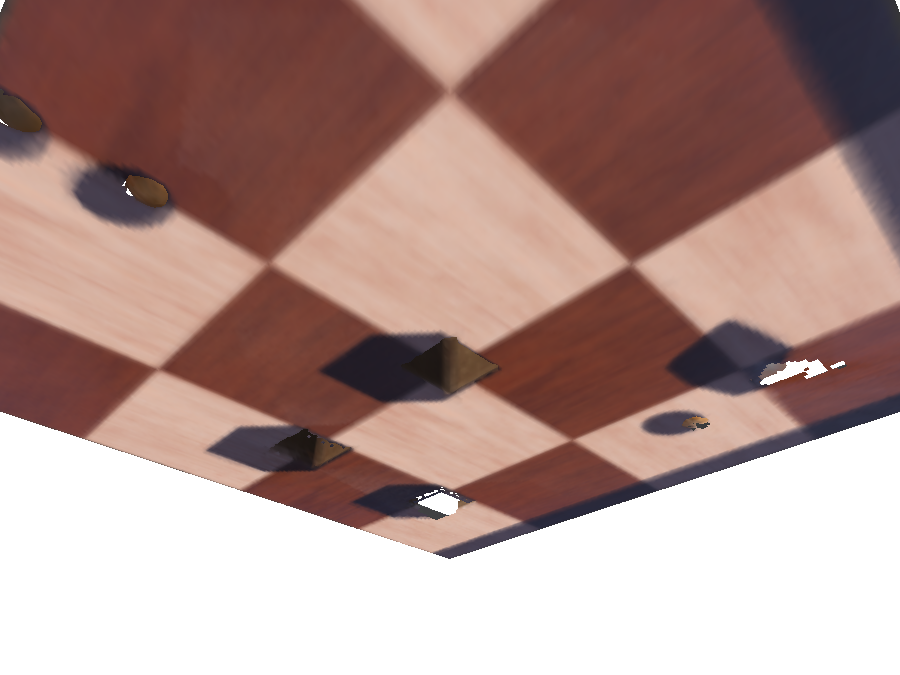
\includegraphics[width=\linewidth]{figures/fig_fused.png}\\
(b) mesh reconstructed by TSDF fusion of 36 frames
\end{minipage}
\caption{Overview of the pipeline studied in this paper: a simulated RGB-D
rig captures color, depth and ground-truth poses along two look-at
trajectories, and the frames are fused into a single consistent 3D model of
the tabletop scene.}
\label{fig:teaser}
\end{figure}

\section{Introduction}

Recovering the 3D structure of a scene from sensor data is a basic skill for
embodied robots: navigation, grasping and simulation modeling all rely on a
geometric model of the world. An RGB-D camera provides, for every pixel, both a
color and a depth value, and the standard pipeline to turn such data into a 3D
model consists of four steps: back-projecting each depth pixel into 3D,
aligning frames captured from different viewpoints using camera poses, fusing
them into a consistent model, and extracting a surface.

Rather than treating this pipeline as a black box, this paper rebuilds it from
first principles and validates every step with a controlled experiment. A
simulated RGB-D camera in Webots provides noise-controllable depth maps and
ground-truth poses, which allows us to check each formula against a known
reference and to run ablation studies under different noise levels.

The contributions are: (1) a derivation of the full pipeline from similar
triangles to TSDF fusion; (2) a Webots data-collection setup with a
look-at trajectory generator that produces pixel-aligned RGB images, depth
maps and ground-truth poses; (3) an experimental validation of the framework
and ablation studies on depth noise, pose noise and voxel size.

\section{Background}

\subsection{The pinhole camera model}

A camera forms an image by projecting 3D points through the optical center $O$
onto an image plane at distance $f$ (the focal length). Let
$P=(X,Y,Z)^\top$ be a point in the camera frame, where $Z$ is measured along
the optical axis. The ray through $O$ intersects the image plane at a point
whose physical coordinates $(x,y)$ follow from similar triangles:
\begin{equation}
\frac{x}{f}=\frac{X}{Z},\qquad \frac{y}{f}=\frac{Y}{Z}
\quad\Longrightarrow\quad
x=f\frac{X}{Z},\quad y=f\frac{Y}{Z}.
\label{eq:similar}
\end{equation}

The image is stored in pixels. If a pixel has physical size $s_x\times s_y$
and the principal point (the intersection of the optical axis with the image
plane) has pixel coordinates $(c_x,c_y)$, the pixel coordinates $(u,v)$ of the
projection are
\begin{equation}
u=\frac{f}{s_x}\frac{X}{Z}+c_x,\qquad
v=\frac{f}{s_y}\frac{Y}{Z}+c_y.
\label{eq:projection}
\end{equation}
The combinations $f_x=f/s_x$ and $f_y=f/s_y$ are the focal lengths expressed in
pixels; they are exactly the values returned by camera calibration or, in a
simulator, by the camera API. In practice $f_x$ is more convenient to derive
from the horizontal field of view $\theta$: since
$\tan(\theta/2)=\frac{W/2}{f_x}$ for an image of width $W$,
\begin{equation}
f_x=\frac{W}{2\tan(\theta/2)},\qquad c_x=\frac{W}{2},\qquad c_y=\frac{H}{2}.
\label{eq:fov}
\end{equation}

\subsection{Depth sensing: from RGB to RGB-D}

Projection \eqref{eq:projection} collapses a whole ray of 3D points onto one
pixel, so a single RGB image loses the depth $Z$ of every point: photography is
a many-to-one mapping that cannot be inverted from color alone. Depth must be
measured separately, e.g.\ by structured light, time-of-flight, stereo
matching, or estimated from the color image itself by a neural network
\cite{densedepth}. Public datasets such as NYU Depth V2 \cite{nyudepth} provide
real aligned RGB-D pairs. An RGB-D camera pairs an RGB sensor with such a depth sensor and
delivers, after alignment, a depth map $D(u,v)$ registered to the color image.
In this work the depth map is produced by a Webots \emph{RangeFinder}, a planar
depth sensor that returns the axial depth $Z$ of the first surface hit by each
pixel's ray (Section~\ref{sec:axial} validates this experimentally). Pixels
whose ray hits nothing within the sensor range return an invalid value
($+\infty$), which must be filtered out.

\section{Method}

\subsection{Single-frame back-projection}

Given a depth map $D(u,v)$ and the intrinsics $(f_x,f_y,c_x,c_y)$,
Eq.~\eqref{eq:projection} is inverted pixel by pixel:
\begin{equation}
Z=D(u,v),\qquad
X=\frac{(u-c_x)\,Z}{f_x},\qquad
Y=\frac{(v-c_y)\,Z}{f_y}.
\label{eq:backproj}
\end{equation}
Every valid pixel yields one 3D point; taking its color from the aligned RGB
image gives a colored point cloud of roughly $2.5\times10^{5}$ points per
$640\times480$ frame.

A practical detail is the coordinate convention. Our Webots sensors follow the
FLU convention: the optical axis is the device $+x$ axis, the image-up
direction is device $+z$, and therefore the image-right direction is
$\text{fwd}\times\text{up}=-y_{\text{dev}}$. Eq.~\eqref{eq:backproj} in device
coordinates thus reads
\begin{equation}
\bm p_{\text{dev}}=
\bigl(Z,\;-\tfrac{(u-c_x)Z}{f_x},\;-\tfrac{(v-c_y)Z}{f_y}\bigr)^\top .
\label{eq:backproj-flu}
\end{equation}

\subsection{From one frame to many: camera poses}

A single frame only captures the surfaces facing the camera; occluded and
back-facing regions are missing. Capturing from several viewpoints requires
knowing where each frame was taken. A camera pose consists of a rotation
$R\in SO(3)$ and a translation $t\in\mathbb{R}^3$, packed into a homogeneous
matrix
\begin{equation}
T=\begin{bmatrix}R & t\\ \bm 0 & 1\end{bmatrix}\in SE(3),
\qquad
\bm p_{\text{world}}=R\,\bm p_{\text{cam}}+t,
\label{eq:pose}
\end{equation}
which maps camera-frame points into a fixed world frame. Padding points with a
fourth coordinate $1$ lets one matrix multiplication perform rotation and
translation at once, and makes poses composable by matrix multiplication. In
our setup the poses are ground truth read from the Webots supervisor; on a real
system they would come from RGB-D odometry and pose-graph optimization.

\subsection{Fusing many point clouds: TSDF}
\label{sec:tsdf}

The naive way to combine $N$ frames is concatenating all back-projected points
in the world frame. This has three problems: every surface is measured $N$
times with independent noise, producing a thickened, rough point fog; the
result contains millions of redundant points; and a point set has no notion of
surface, so it cannot directly produce a mesh.

TSDF fusion \cite{kinectfusion} replaces points with a scalar field. Space is divided into voxels;
each voxel stores a truncated signed distance $D$ to the nearest surface
(positive in front, negative behind) and a weight $W$. Only voxels within a
truncation margin $\pm\mu$ of a measured surface are updated. For each frame, a
voxel is projected into the depth map using the inverse pose
$\bm p_{\text{cam}}=T^{-1}\bm p_{\text{world}}$; with the measured depth
$z_{\text{meas}}$ and the voxel's own depth $z_{\text{vox}}$, the observation
is $d=z_{\text{meas}}-z_{\text{vox}}$, truncated to $[-\mu,\mu]$. The voxel is
updated by an incremental weighted average
\begin{equation}
D\leftarrow\frac{W D+w\,d}{W+w},\qquad W\leftarrow W+w,
\label{eq:tsdf}
\end{equation}
so $N$ noisy votes of the same voxel cancel out as $N$ grows. The surface is
the zero level set $\{\bm x:D(\bm x)=0\}$, extracted as a triangle mesh by
marching cubes \cite{marchingcubes}: for each cell whose eight corner voxels change sign, the zero
crossing on every sign-changing edge is linearly interpolated and connected
into triangles from a 256-case lookup table; interpolation places the surface
with sub-voxel precision. Our implementation builds on Open3D's
\emph{ScalableTSDFVolume} \cite{open3d}.

\subsection{Data collection in Webots}

The scene is a $1\,\mathrm{m}\times1\,\mathrm{m}$ tabletop arena \cite{webots}
containing
three boxes, three balls and a rock (Fig.~\ref{fig:world}). A robot node
carries a $640\times480$ color camera and a $640\times480$ RangeFinder with
identical field of view, so the two images are pixel-aligned by construction.
A supervisor controller moves the rig along two circular look-at trajectories
(radius $0.65\,\mathrm{m}$ at height $0.50\,\mathrm{m}$ and radius
$0.50\,\mathrm{m}$ at height $0.25\,\mathrm{m}$, 18 frames each), always facing
the scene center, and stores RGB, depth and the ground-truth pose per frame.

\begin{figure}[H]
\centering
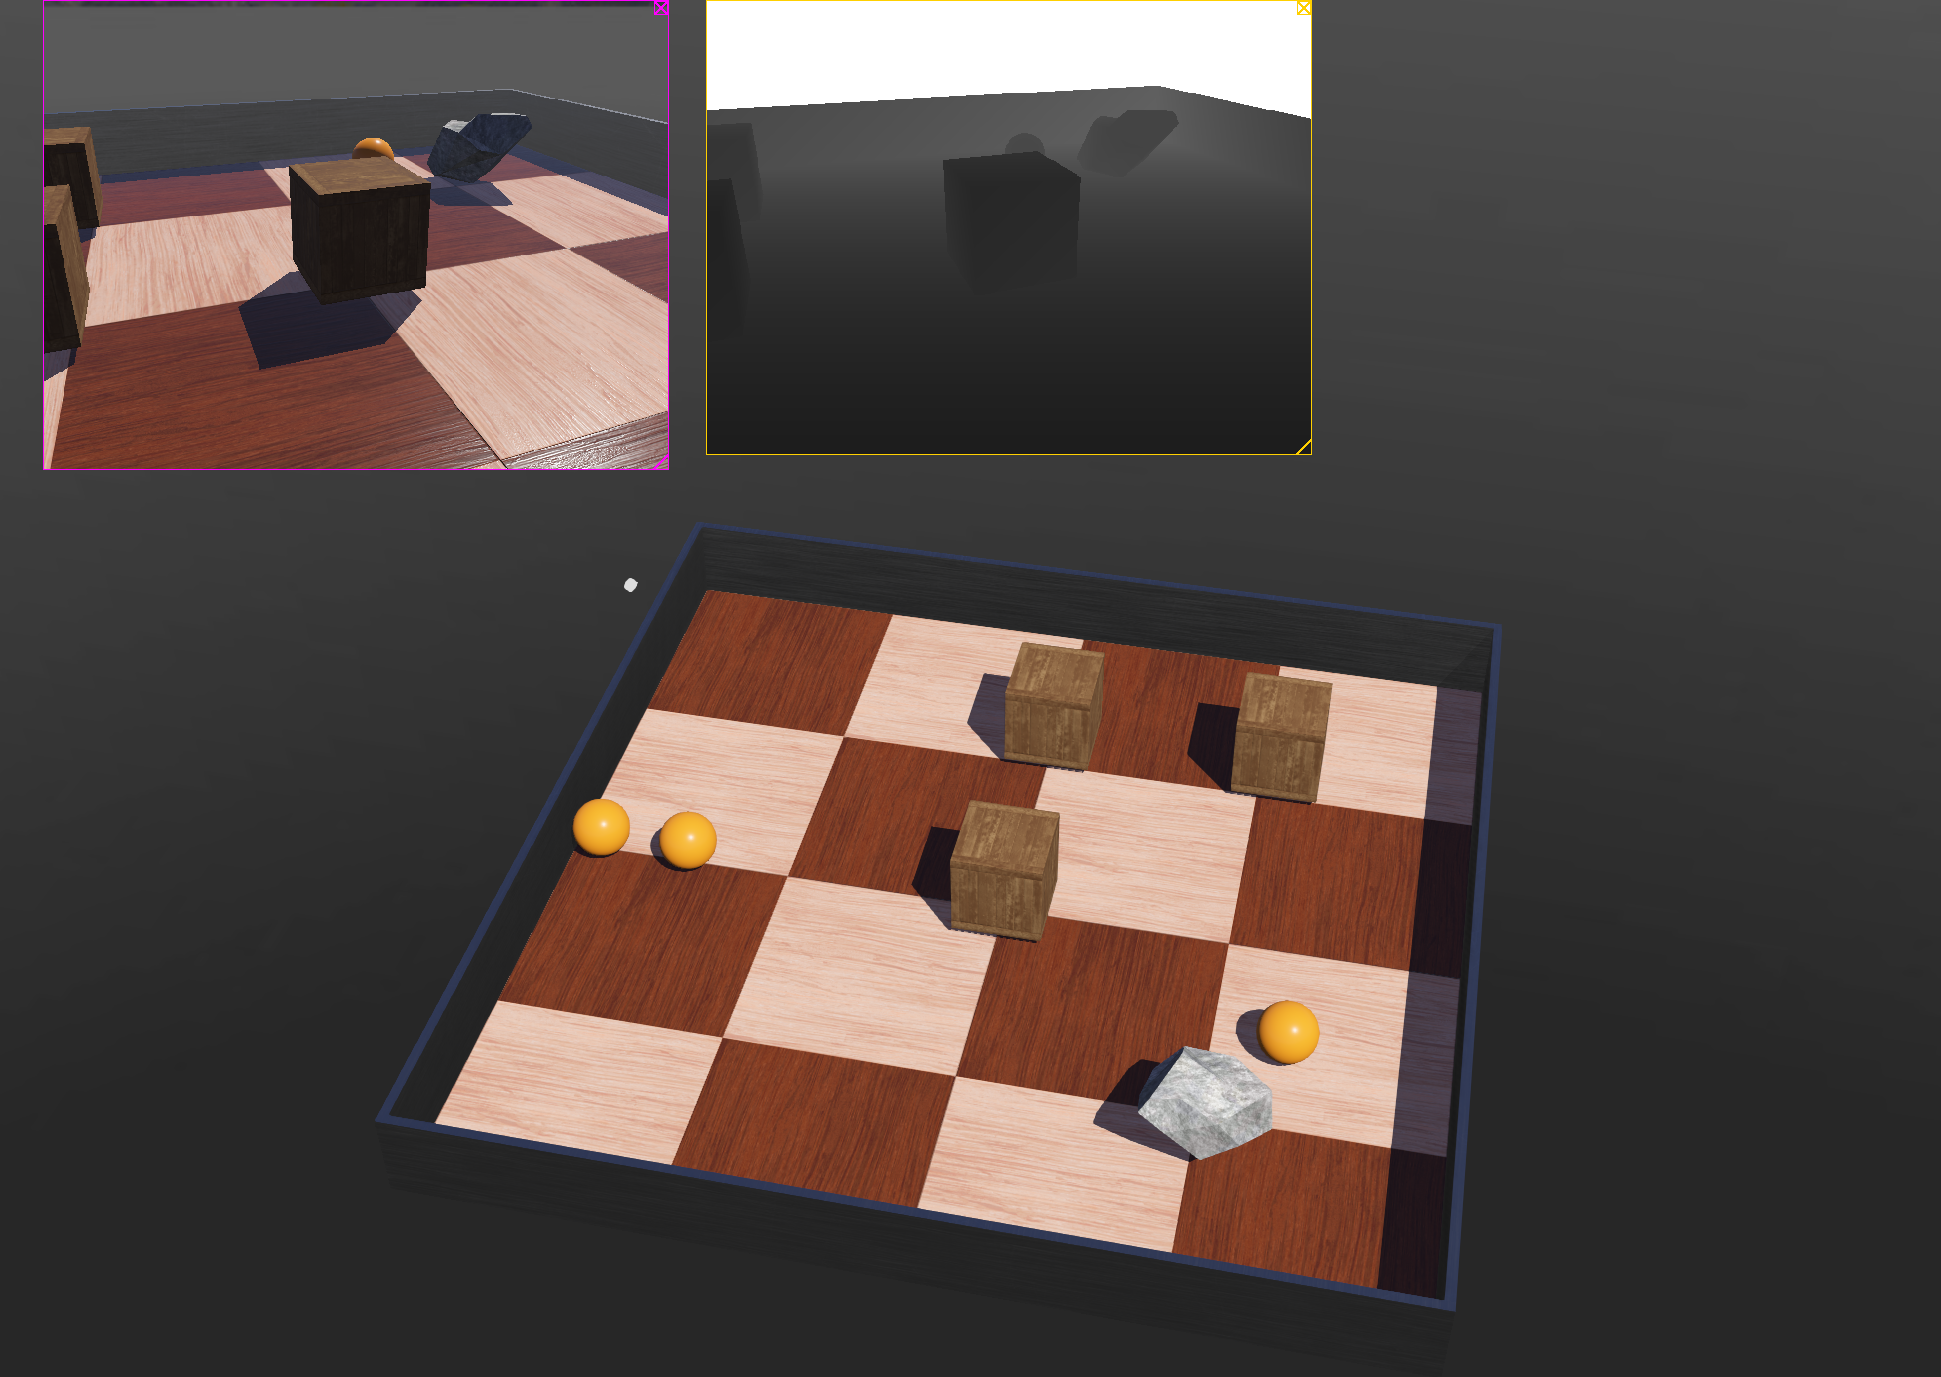
\includegraphics[width=0.65\linewidth]{figures/fig_world.png}
\caption{The Webots tabletop scene: a $1\,\mathrm{m}\times1\,\mathrm{m}$ arena
with three boxes, three balls and a rock. The sensor rig (camera $+$
RangeFinder) moves on two circular look-at trajectories around the center.}
\label{fig:world}
\end{figure}

\section{Experiments}
\label{sec:exp}

\subsection{Experimental setup}

All experiments use the 36-frame dataset described above. The reference metric
is the \emph{floor flatness}: the true floor is the plane $z=0$, so for a
reconstruction we take vertices inside the arena ($|x|,|y|<0.45\,\mathrm{m}$)
within $\pm2\,\mathrm{cm}$ of the floor median and report the RMS of their $z$
residuals. Unless stated otherwise, TSDF uses $5\,\mathrm{mm}$ voxels and a
$20\,\mathrm{mm}$ truncation margin.

\subsection{Framework validation}
\label{sec:validation}

\textbf{Intrinsics.} Eq.~\eqref{eq:fov} predicts
$f_x=640/(2\tan 0.3925)=772.6$ px for the initial $\theta=0.785$ rad camera;
the simulator API returns $772.55$ px ($0.06\%$ error). For the widened
$\theta=1.0$ rad camera it predicts $585.8$ px vs.\ $585.76$ px measured.

\textbf{Axial vs.\ radial depth.} If the RangeFinder returned ray (radial)
distances $d$ instead of axial depths $Z$, a correction
$Z=d/\sqrt{1+\tilde u^2+\tilde v^2}$ would be required. Back-projecting without
correction leaves $77.6\%$ of points within $2\,\mathrm{cm}$ of the floor
plane; applying the correction bends the flat floor upward and drops the ratio
to $26.9\%$. The sensor therefore already outputs axial depth, consistent with
its planar projection model.

\textbf{Single frame vs.\ fusion.} A single back-projected frame covers only
the surfaces facing the camera (Fig.~\ref{fig:single}). Fusing 36 frames yields
a $67{,}588$-vertex mesh spanning $x,y\in[-0.51,0.51]\,\mathrm{m}$ and
$z\in[0,0.11]\,\mathrm{m}$, matching the true arena exactly, with a floor RMS
of $2.7\,\mathrm{mm}$.

\begin{figure}[H]
\centering
\begin{minipage}{0.48\linewidth}
\centering
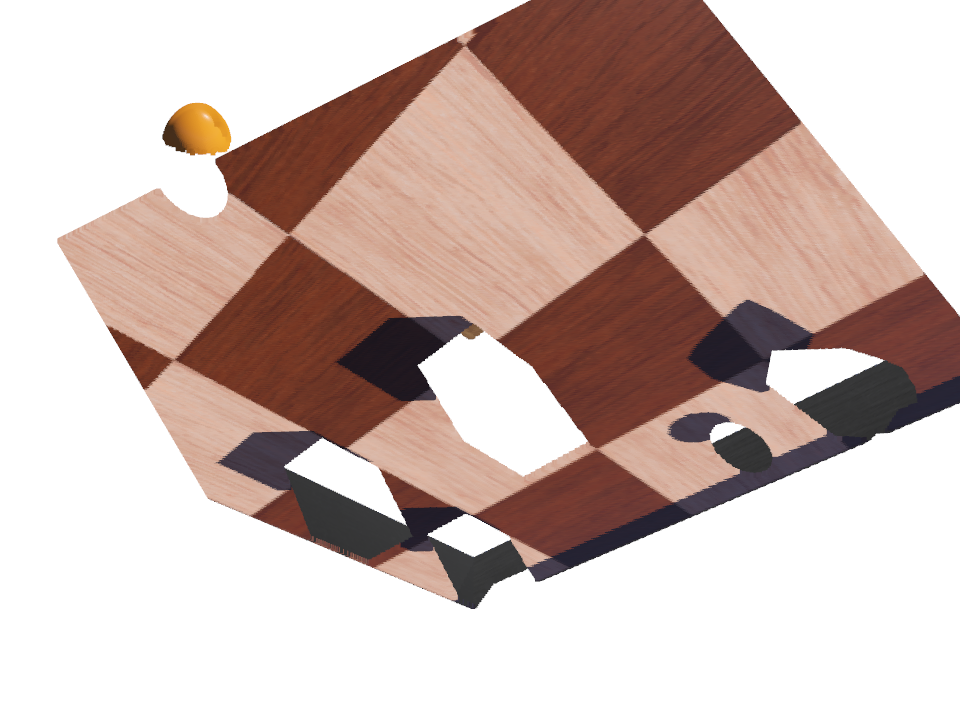
\includegraphics[width=\linewidth]{figures/fig_single.png}\\
(a) single frame, one viewpoint
\end{minipage}\hfill
\begin{minipage}{0.48\linewidth}
\centering
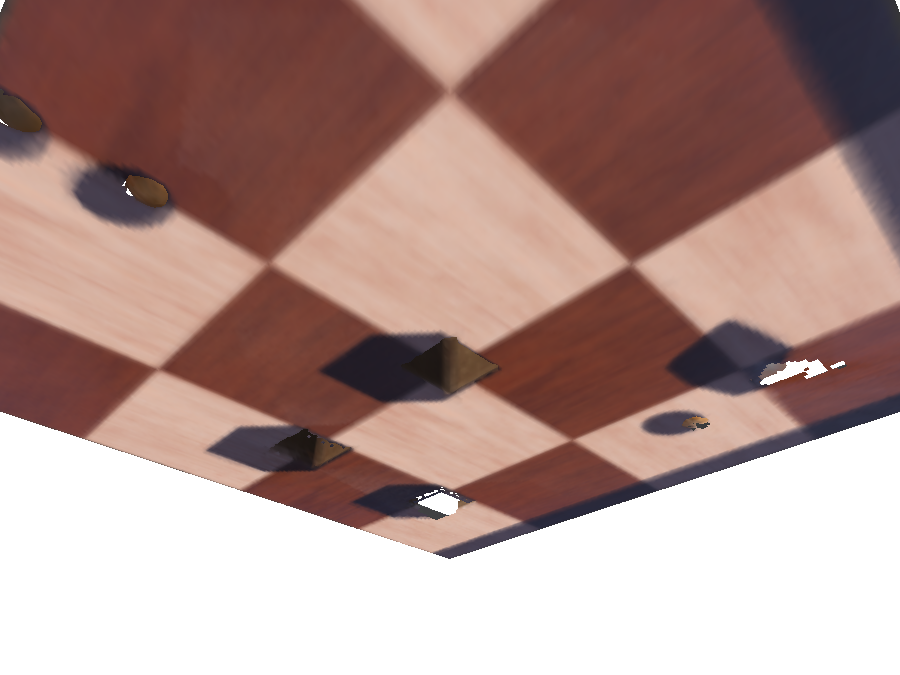
\includegraphics[width=\linewidth]{figures/fig_fused.png}\\
(b) TSDF fusion of all 36 frames
\end{minipage}
\caption{Single-frame coverage vs.\ fused reconstruction. A single
back-projected frame covers only the surfaces facing the camera; the fused
mesh is complete and spans exactly the true arena.}
\label{fig:single}
\end{figure}

\subsection{Ablation: depth noise}
\label{sec:depthnoise}

To emulate a real RGB-D sensor we add zero-mean Gaussian noise of standard
deviation $\sigma\in\{0,2,5,10,20\}\,\mathrm{mm}$ to every valid depth pixel
and compare naive concatenation (voxel-downsampled at $5\,\mathrm{mm}$) with
TSDF fusion (Table~\ref{tab:depthnoise}, Fig.~\ref{fig:noise}a).

\begin{table}[H]
\centering
\caption{Floor RMS residual under depth noise (lower is better).}
\label{tab:depthnoise}
\begin{tabular}{cccc}
\toprule
$\sigma$ (mm) & Direct merge (mm) & TSDF (mm) & TSDF vertices \\
\midrule
0  & 2.77  & 2.68 & 67{,}588 \\
2  & 2.96  & 2.69 & 67{,}690 \\
5  & 6.26  & 2.75 & 72{,}873 \\
10 & 10.36 & 4.10 & 106{,}202 \\
20 & 11.58 & 7.03 & 345{,}902 \\
\bottomrule
\end{tabular}
\end{table}

\begin{figure}[H]
\centering
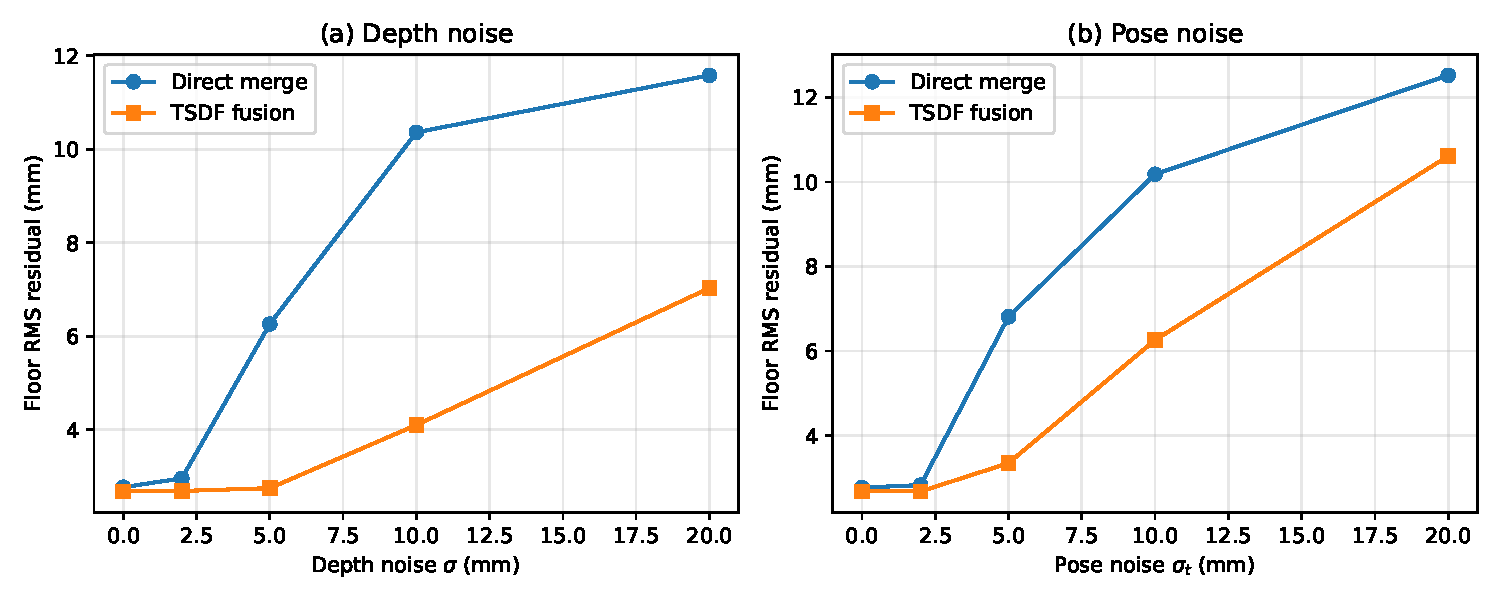
\includegraphics[width=0.62\linewidth]{figures/fig_noise.pdf}
\caption{Floor RMS residual vs.\ noise level for naive concatenation and TSDF
fusion: (a) depth noise, (b) pose noise. In both cases the methods are
equivalent with clean data, while beyond a few millimetres of noise TSDF
absorbs much of the error through the running average \eqref{eq:tsdf}.}
\label{fig:noise}
\end{figure}

\subsection{Ablation: pose noise}
\label{sec:posenoise}

Ground-truth poses are perturbed by Gaussian translation noise of standard
deviation $\sigma_t$ and a random-axis rotation of standard deviation
$\sigma_t/10$ (Table~\ref{tab:posenoise}, Fig.~\ref{fig:noise}b).

\begin{table}[H]
\centering
\caption{Floor RMS residual under pose noise.}
\label{tab:posenoise}
\begin{tabular}{ccc}
\toprule
$\sigma_t$ (mm) & Direct merge (mm) & TSDF (mm) \\
\midrule
0  & 2.77  & 2.68 \\
2  & 2.83  & 2.68 \\
5  & 6.81  & 3.35 \\
10 & 10.18 & 6.26 \\
20 & 12.52 & 10.61 \\
\bottomrule
\end{tabular}
\end{table}

\subsection{Ablation: voxel size}
\label{sec:voxel}

\begin{table}[H]
\centering
\caption{Voxel size vs.\ quality and runtime (36 frames).}
\label{tab:voxel}
\begin{tabular}{cccc}
\toprule
Voxel (mm) & Vertices & Floor RMS (mm) & Time (s) \\
\midrule
2  & 466{,}672 & 2.55 & 2.8 \\
5  & 67{,}588  & 2.68 & 0.7 \\
10 & 16{,}620  & 2.68 & 0.3 \\
20 & 4{,}226   & 3.16 & 0.2 \\
\bottomrule
\end{tabular}
\end{table}

\begin{figure}[H]
\centering
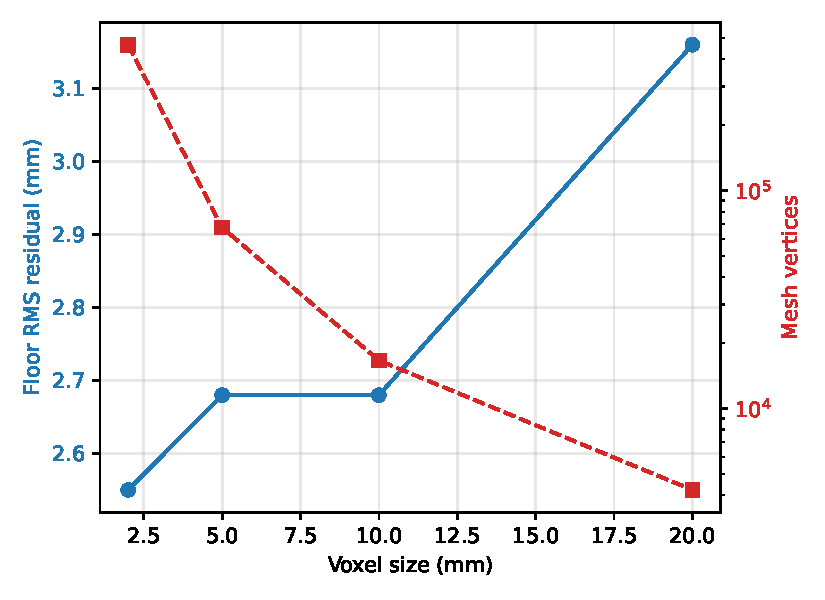
\includegraphics[width=0.62\linewidth]{figures/fig_voxel.pdf}
\caption{Voxel size vs.\ mesh size and floor RMS. Between $2$ and
$10\,\mathrm{mm}$ the floor metric is almost unchanged while the vertex count
drops by a factor of $7$; the loss of fine detail at larger voxels shows up at
object edges rather than on the flat floor.}
\label{fig:voxel}
\end{figure}

\subsection{Discussion}

\textbf{Depth noise.} With clean depth both methods are equivalent
($2.77$ vs.\ $2.68\,\mathrm{mm}$), which is expected: the simulator sensor is
exact, so there is nothing to average away. As $\sigma$ grows, naive
concatenation keeps every noisy sample, so the floor residual tracks the noise
level almost linearly ($10.36\,\mathrm{mm}$ at $\sigma=10\,\mathrm{mm}$) and
the $5\,\mathrm{mm}$ downsampling grid can no longer deduplicate the thickened
surface ($67\mathrm{k}\to838\mathrm{k}$ points). TSDF fusion stays nearly flat
up to $\sigma=5\,\mathrm{mm}$ and degrades gracefully afterwards
($4.10/7.03\,\mathrm{mm}$ at $\sigma=10/20\,\mathrm{mm}$). The price shows in
the vertex count ($67\mathrm{k}\to346\mathrm{k}$): with large noise the running
average no longer cancels the error completely, and the zero level set becomes
a rougher, slightly thickened surface that marching cubes samples more
densely.

\textbf{Pose noise.} TSDF is better at every non-zero level
($3.35$ vs.\ $6.81\,\mathrm{mm}$ at $\sigma_t=5\,\mathrm{mm}$). Pose errors
shift whole frames coherently, so the same surface lands in slightly different
voxels per frame; the weighted average still pulls the zero level set toward
the centroid of the votes, while concatenation keeps all copies side by side.
At $\sigma_t=20\,\mathrm{mm}$ both methods degrade noticeably
($12.52/10.61\,\mathrm{mm}$): pose error is systematic per frame, and no amount
of per-voxel averaging fully recovers structure that was never observed from
the right place.

\textbf{Voxel size.} Between $2$ and $10\,\mathrm{mm}$ the floor RMS is
essentially constant ($2.55$--$2.68\,\mathrm{mm}$) while the vertex count drops
from $467\mathrm{k}$ to $17\mathrm{k}$ and runtime from $2.8$ to $0.3$ s. This
partly reflects a limitation of the metric: the floor is flat and large, so
marching-cubes interpolation recovers it well at any of these resolutions. The
real cost of coarse voxels appears at object edges and thin structures, which
blur once the voxel size approaches their thickness; the jump in RMS at
$20\,\mathrm{mm}$ ($3.16\,\mathrm{mm}$) hints at this. For this scene,
$5\,\mathrm{mm}$ is a good balance.

\textbf{Limitations.} All experiments use ground-truth poses and a synthetic
sensor; a real system must estimate poses online (RGB-D odometry plus
pose-graph optimization), where drift interacts with fusion in ways not
captured here. The floor-RMS metric captures planarity but not completeness or
fine detail, and the look-at trajectory gives near-ideal coverage that a real
robot rarely has.

\section{Conclusion}

We rebuilt the RGB-D reconstruction pipeline from first principles and
validated every stage experimentally in Webots. The pinhole model follows from
similar triangles and predicts the simulator intrinsics within $0.1\%$; a depth
measurement turns the non-invertible projection into an invertible one, giving
a colored point cloud per frame; poses align frames into a common world frame;
and TSDF fusion merges the noisy, redundant clouds into a consistent surface,
extracted by marching cubes. On clean simulated data the fused mesh reproduces
the $1\,\mathrm{m}\times1\,\mathrm{m}$ scene exactly with a floor RMS of
$2.7\,\mathrm{mm}$. Ablations confirm that fusion is unnecessary when the
sensor is perfect but increasingly valuable as depth or pose noise grows, and
that $5\,\mathrm{mm}$ voxels balance quality, size and runtime for this scene.
The natural next step is replacing ground-truth poses with estimated ones,
closing the loop toward a fully self-contained real-to-sim reconstruction
pipeline.

\begin{thebibliography}{9}

\bibitem{kinectfusion}
R.~A. Newcombe, S.~Izadi, O.~Hilliges, D.~Molyneaux, D.~Kim, A.~J. Davison,
P.~Kohli, J.~Shotton, S.~Hodges, and A.~Fitzgibbon,
``KinectFusion: Real-time dense surface mapping and tracking,''
in \emph{Proc. IEEE ISMAR}, 2011, pp. 127--136.

\bibitem{marchingcubes}
W.~E. Lorensen and H.~E. Cline,
``Marching cubes: A high resolution 3D surface construction algorithm,''
\emph{ACM SIGGRAPH Computer Graphics} (Proc.\ SIGGRAPH), vol.~21, no.~4,
pp.~163--169, 1987.

\bibitem{nyudepth}
N.~Silberman, D.~Hoiem, P.~Kohli, and R.~Fergus,
``Indoor segmentation and support inference from RGBD images,''
in \emph{Proc. ECCV}, 2012, pp. 746--760.

\bibitem{open3d}
Q.-Y. Zhou, J.~Park, and V.~Koltun,
``Open3D: A modern library for 3D data processing,''
\emph{arXiv:1801.09847}, 2018.

\bibitem{webots}
O.~Michel,
``Webots: Professional mobile robot simulation,''
\emph{International Journal of Advanced Robotic Systems}, vol.~1, no.~1,
pp.~39--42, 2004.

\bibitem{densedepth}
I.~Alhashim and P.~Wonka,
``High quality monocular depth estimation via transfer learning,''
\emph{arXiv:1812.11941}, 2018.

\end{thebibliography}

\end{document}
